% ============PREAMBLE SECTION==========================================
%+++++++++++++++++++++++++++++++++++++++++++++++++++++++++++++++++++++++
\documentclass[12pt]{article}
\usepackage{geometry}                % See geometry.pdf to learn the layout options. There are lots.
\geometry{letterpaper}                   % ... or a4paper or a5paper or ... 
%\geometry{landscape}                % Activate for for rotated page geometry
\usepackage[parfill]{parskip}    % Activate to begin paragraphs with an empty line rather than an indent
\usepackage{daves,fancyhdr,natbib,graphicx,dcolumn,amsmath,lastpage,url}
\usepackage{amsmath,amssymb,epstopdf,longtable}
\DeclareGraphicsRule{.tif}{png}{.png}{`convert #1 `dirname #1`/`basename #1 .tif`.png}
\pagestyle{fancy}
\lhead{Student Name: \_\_\_\_\_\_\_\_\_\_\_\_\_\_\_\_\_\_\_\_\_\_\_\_\_\_\_\_\_\_\_\_\_\_\_\_\_\_\_\_\_\_\_\_\_ }
\rhead{FALL 2024}
\lfoot{CE 3354 Engineering Hydrology }
\cfoot{EXAM 3}
\rfoot{Page \thepage\ of \pageref{LastPage}}
\renewcommand\headrulewidth{0pt}

% other
\usepackage{paralist}  % need to modify standard enumerate blocks
%=========Longtable environment
\usepackage{setspace}                % allow single and double space environment
\usepackage{longtable}                % allow table to span multiple pages
\usepackage{caption}                    % consistent caption package
\usepackage{url}					% Ubiquitious url formatting package
%===========

\DeclareGraphicsRule{.tif}{png}{.png}{`convert #1 `dirname #1`/`basename #1 .tif`.png}
%++++++++++++++++++++++++++++++++++++++++++++++++++++++++++++++++++++++++++
%============================================================================
\begin{document}

\begingroup
\begin{centering}
\textbf{CE 3354 Engineering Hydrology} \\
\textbf{Exam 3, FALL 2024}\\
\end{centering}
~\\
The exam is to be completed on Blackboard. The questions below are the same as on the Blackboard implementation.
\endgroup

\begin{enumerate}

%%%%%%%%%%%%%%%%%%%%%%%%%%%
%\item Which of the following is a hyetograph (as used in this class)?
%\begin{enumerate}[a)]
%\item A record of infiltration rates (inches/hour) versus time.
%\item A record of cumulative rainfall depth (inches) versus time.
%\item A record of discharge rate (cubic feet/second) versus time.
%\item A and B
%\end{enumerate}
%%%%%%%%%%%%%%%%%%%%%%%%%%%%
\item What is a hydrograph (as used in this class)?
\begin{enumerate}[a)]
\item A record of rainfall rates (inches/hour) versus time.
\item A record of cumulative rainfall depth (inches) versus time.
\item A record of discharge rate (cubic feet/second) versus time.
\item A and B
\end{enumerate}
\clearpage
%%%%%%%%%%%%%%%%%%%%%%%%%%%%
\item What is excess precipitation?
\begin{enumerate}[a)]
\item The amount of precipitation that falls upon a watershed.
\item The amount of runoff that is produced from a watershed.
\item The equivalent depth of uniformly distributed precipitation.
\item A and B
\end{enumerate}
\clearpage
%%%%%%%%%%%%%%%%%%%%%%%%%%%%
\item Hydrology is
\begin{enumerate}[a)]
\item Study of the atmosphere, ocean, and surface waters
\item The study of the occurrence, distribution, and movement of water above, on, and below the surface of the earth
\item A study of the processes of evaporation, infiltration, and storage
\item The study of the relationship between rainfall and runoff
\end{enumerate}
\clearpage

%%%%%%%%%%%%%%%%%%%%%%%%%%%
%\item To what type of data series would we apply the Bulletin 17B procedure ?
%\begin{enumerate}[a)]
%\item Instantaneous discharge
%\item Hourly rainfall
%\item Annual maximum rainfall
%\item Annual maximum discharge
%\end{enumerate}
%%%%%%%%%%%%%%%%%%%%%%%%%%%%%%
\item Rainfall behavior is expressed as a combination of 
\begin{enumerate}[a)]
\item depth or intensity, duration, and probability or frequency
\item intensity and probability or frequency
\item duration and probability or frequency
\item depth and duration
\end{enumerate}
\clearpage
%%%%%%%%%%%%%%%%%%%%%%%%%%%%%%%%%%
%\item How can one calculate the Annual Exceedance Probability (AEP) from the Annual Return Interval (ARI)?
%\begin{enumerate}[a)]
%\item	$AEP = \frac{1~yr}{ARI}$
%\item	$ARI = \frac{1~yr}{AEP}$
%\item	$ARI = \frac{Rank_i}{N+1}$
%\item	Cannot
%\end{enumerate}
%%%%%%%%%%%%%%%%%%%%%%%%%%%%%%%%%%%%%
\item An annual recurrence interval of 100-years is equivalent to an Annual Exceedance Probability (AEP) of what percent?
\begin{enumerate}[a)]
\item 1-percent.
\item 10-percent.
\item 50-percent.
\item 100-percent.
\end{enumerate}
\clearpage
%%%%%%%%%%%%%%%%%%%%%%%%%%%%%%%%%%%
\item What is a plotting position?
\begin{enumerate}[a)]
\item The multiplicative inverse of relative frequency
\item An estimate of probability associated with an observation based on its magnitude relative to the arithmetic mean
\item An estimate of probability associated with an observation based on its position within a ranked sample set
\item Location in a chart of a data pair
\end{enumerate}
\clearpage
%%%%%%%%%%%%%%%%%%%%%%%%%%%%%%%%%%%%%
\item What is a flood frequency curve?
\begin{enumerate}[a)]
\item A plot of discharge and time
\item A plot of estimated exceedance probability and discharge
\item A plot of the frequency and discharge
\item A plot of the discharge magnitude and the Weibull plotting position
\end{enumerate}
\clearpage
%%%%%%%%%%%%%%%%%%%%%%%%%%%%%%%%%%%
\item Average rainfall intensity is 
\begin{enumerate}[a)]
\item instantaneous rainfall rate
\item slope of the depth duration curve at a duration of one hour
\item the ratio of accumulated depth to duration
\item integral of the depth duration curve from 0 to 24 hours
\end{enumerate}
\clearpage
%%%%%%%%%%%%%%%%%%%%%%%%%%%%%%%%%%%
\item In the rational equation, Q = CIA, the intensity, I, is
\begin{enumerate}[a)]
\item the ratio of depth to the time of concentration
\item the ratio of depth to watershed area
\item the ratio of depth to storm duration
\item the ratio of depth to watershed impervious cover
\end{enumerate}
\clearpage

\item The rational runoff coefficient for a 300 X 200-meter property with a slope of 3\% is 0.35. The rainfall intensity is 116 mm/hr. The peak discharge from this property is anticipated to be about

\begin{enumerate}[a)]
\item $2200~\frac{m^3}{hr}$
\item $2400~\frac{m^3}{hr}$%thisone
\item $3800~\frac{m^3}{hr}$
\item $7000~\frac{m^3}{hr}$
\end{enumerate}
\clearpage

\item A 3.2-inch storm is uniformly distributed over a 95 acre watershed. The NRCS Curve Number for the watershed is CN = 78. The anticipated watershed runoff is about

\begin{enumerate}[a)]
\item $8.0$~acre-feet
\item $9.0$~acre-feet
\item $10.0$~acre-feet%thisone
\item $11.0$~acre-feet
\end{enumerate}
\clearpage

\item A 3.5 acre drainage area receives a rainfall intensity of 0.5 in/hour; the peak runoff from the area is 500 gallons per minute. What is the runoff coefficient?
%standard answer set
\begin{enumerate} [(A)]
\item 0.11
\item 0.31
\item 0.64 %thisone
\item 0.86
\end{enumerate}
\clearpage

\item A residential lot of 0.37 acres contains a house that occupies 0.05 acres, and a driveway that covers 0.035 acres. The runoff coefficients are 0.50 for the undeveloped portions of the lot, 0.85 for the house, and 0.90 for the driveway. The peak discharge from the lot during a storm event with rainfall intensity of 0.5 inches per hour is 
%standard answer set
\begin{enumerate}[(A)]
\item $0.085$ $\text{ft}^3/\text{sec}$
\item $0.110$ $\text{ft}^3/\text{sec}$
\item $0.250$ $\text{ft}^3/\text{sec}$
\item $0.320$ $\text{ft}^3/\text{sec}$
\end{enumerate}
\clearpage

\item In an area with a composite runof coeflicient of 0.65, the surface runoff flows toward a steet from the land on both sides. The watershed area extends to 100 ft on eaoh side of the street centerline. The street has curb-and-gutter, and there is a curb inlet (or basin) on both sides of the street The capacity of the curb inlet to pick up runoff from the gutter is 10 cfs (any more than this will just run past the opening). City policy is to design the street drainage system to acoommodate a 6.8-in/hr rainfall. The distance (ft) between the inlets along the sheet should be most nearly:

\begin{enumerate}[a)]
\item $230$~feet
\item $490$~feet
\item $640$~feet
\item $980$~feet
\end{enumerate}

\clearpage
%%%%%%%%%%%%%%%%%%%%%%%%%%%
% HEC-HMS Questions
%%%%%%%%%%%%%%%%%%%%%%%%%%%
Figure \ref{fig:HEC-HMS-Output2} is a screen capture of a HEC-HMS model run.

\begin{figure}[h!] %  figure placement: here, top, bottom, or page
   \centering
   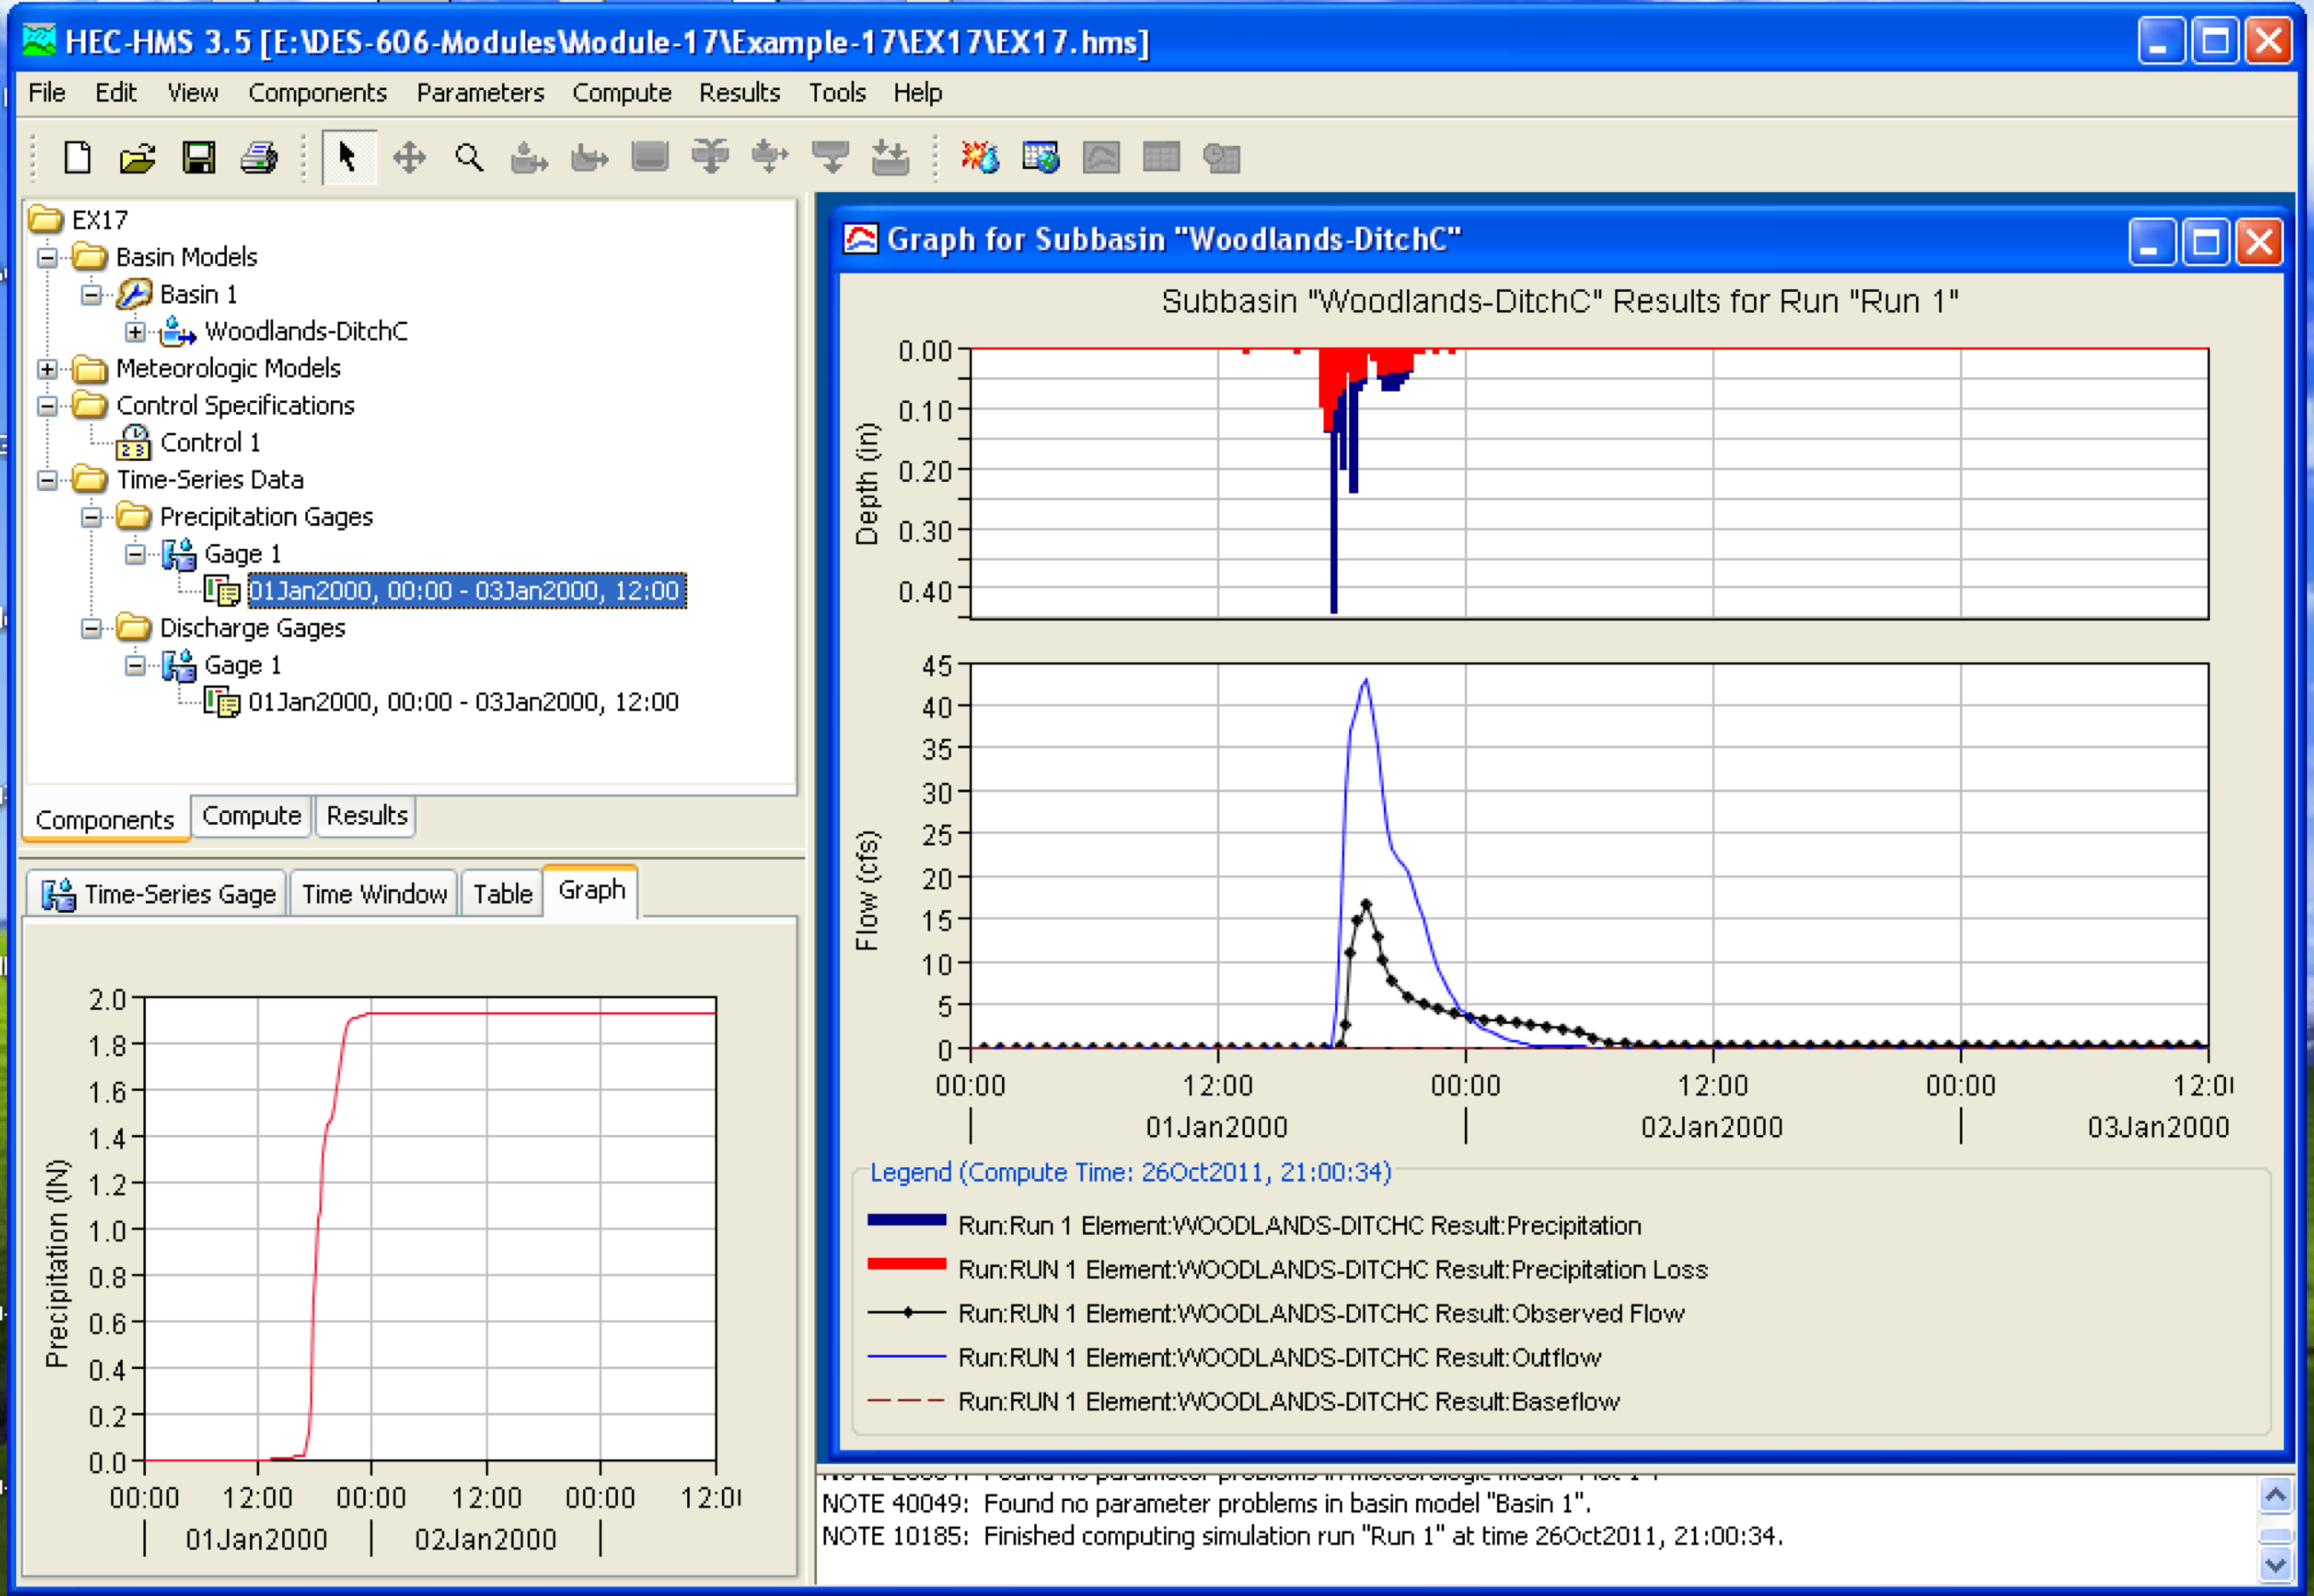
\includegraphics[width=6in]{HEC-HMS-Output2.jpg} 
   \caption{HEC-HMS Model Run for Woodlands-Ditch C sub-basin.}
   \label{fig:HEC-HMS-Output2}
\end{figure}

\item Which value below is the best estimate of the \textbf{COMPUTED} peak discharge for the Woodlands-DitchC sub-basin based upon Figure \ref{fig:HEC-HMS-Output2}?

\begin{enumerate}[a)]
\item $0.5$~inches
\item $1.9$~inches
\item $19$~cubic feet per second
\item $44$~cubic feet per second
\end{enumerate}

\clearpage
\item Which value below is the best estimate of the \textbf{OBSERVED} peak discharge for the Woodlands-DitchC sub-basin based upon Figure \ref{fig:HEC-HMS-Output2}?

\begin{enumerate}[a)]
\item $0.5$~inches
\item $1.9$~inches
\item $19$~cubic feet per second
\item $44$~cubic feet per second
\end{enumerate}

\clearpage
\item Which value below is the best estimate of the total \textbf{RAW} input precipitation for the Woodlands-DitchC sub-basin based upon Figure \ref{fig:HEC-HMS-Output2}?

\begin{enumerate}[a)]
\item $0.5$~inches
\item $1.9$~inches
\item $19$~cubic feet per second
\item $44$~cubic feet per second
\end{enumerate}

\clearpage
\item Which value below is the best estimate of the total \textbf{EXCESS} input precipitation for the Woodlands-DitchC sub-basin based upon Figure \ref{fig:HEC-HMS-Output2}?

\begin{enumerate}[a)]
\item $0.5$~inches
\item $1.9$~inches
\item $19$~cubic feet per second
\item $44$~cubic feet per second
\end{enumerate}

\clearpage
\item Figure \ref{fig:HEC-HMS-Output3} is a screen capture of a HEC-HMS model run.  The model appears to have successfully run, but when the output graph is selected there in no hyetograph nor hydrograph displayed.

\begin{figure}[h!] %  figure placement: here, top, bottom, or page
   \centering
   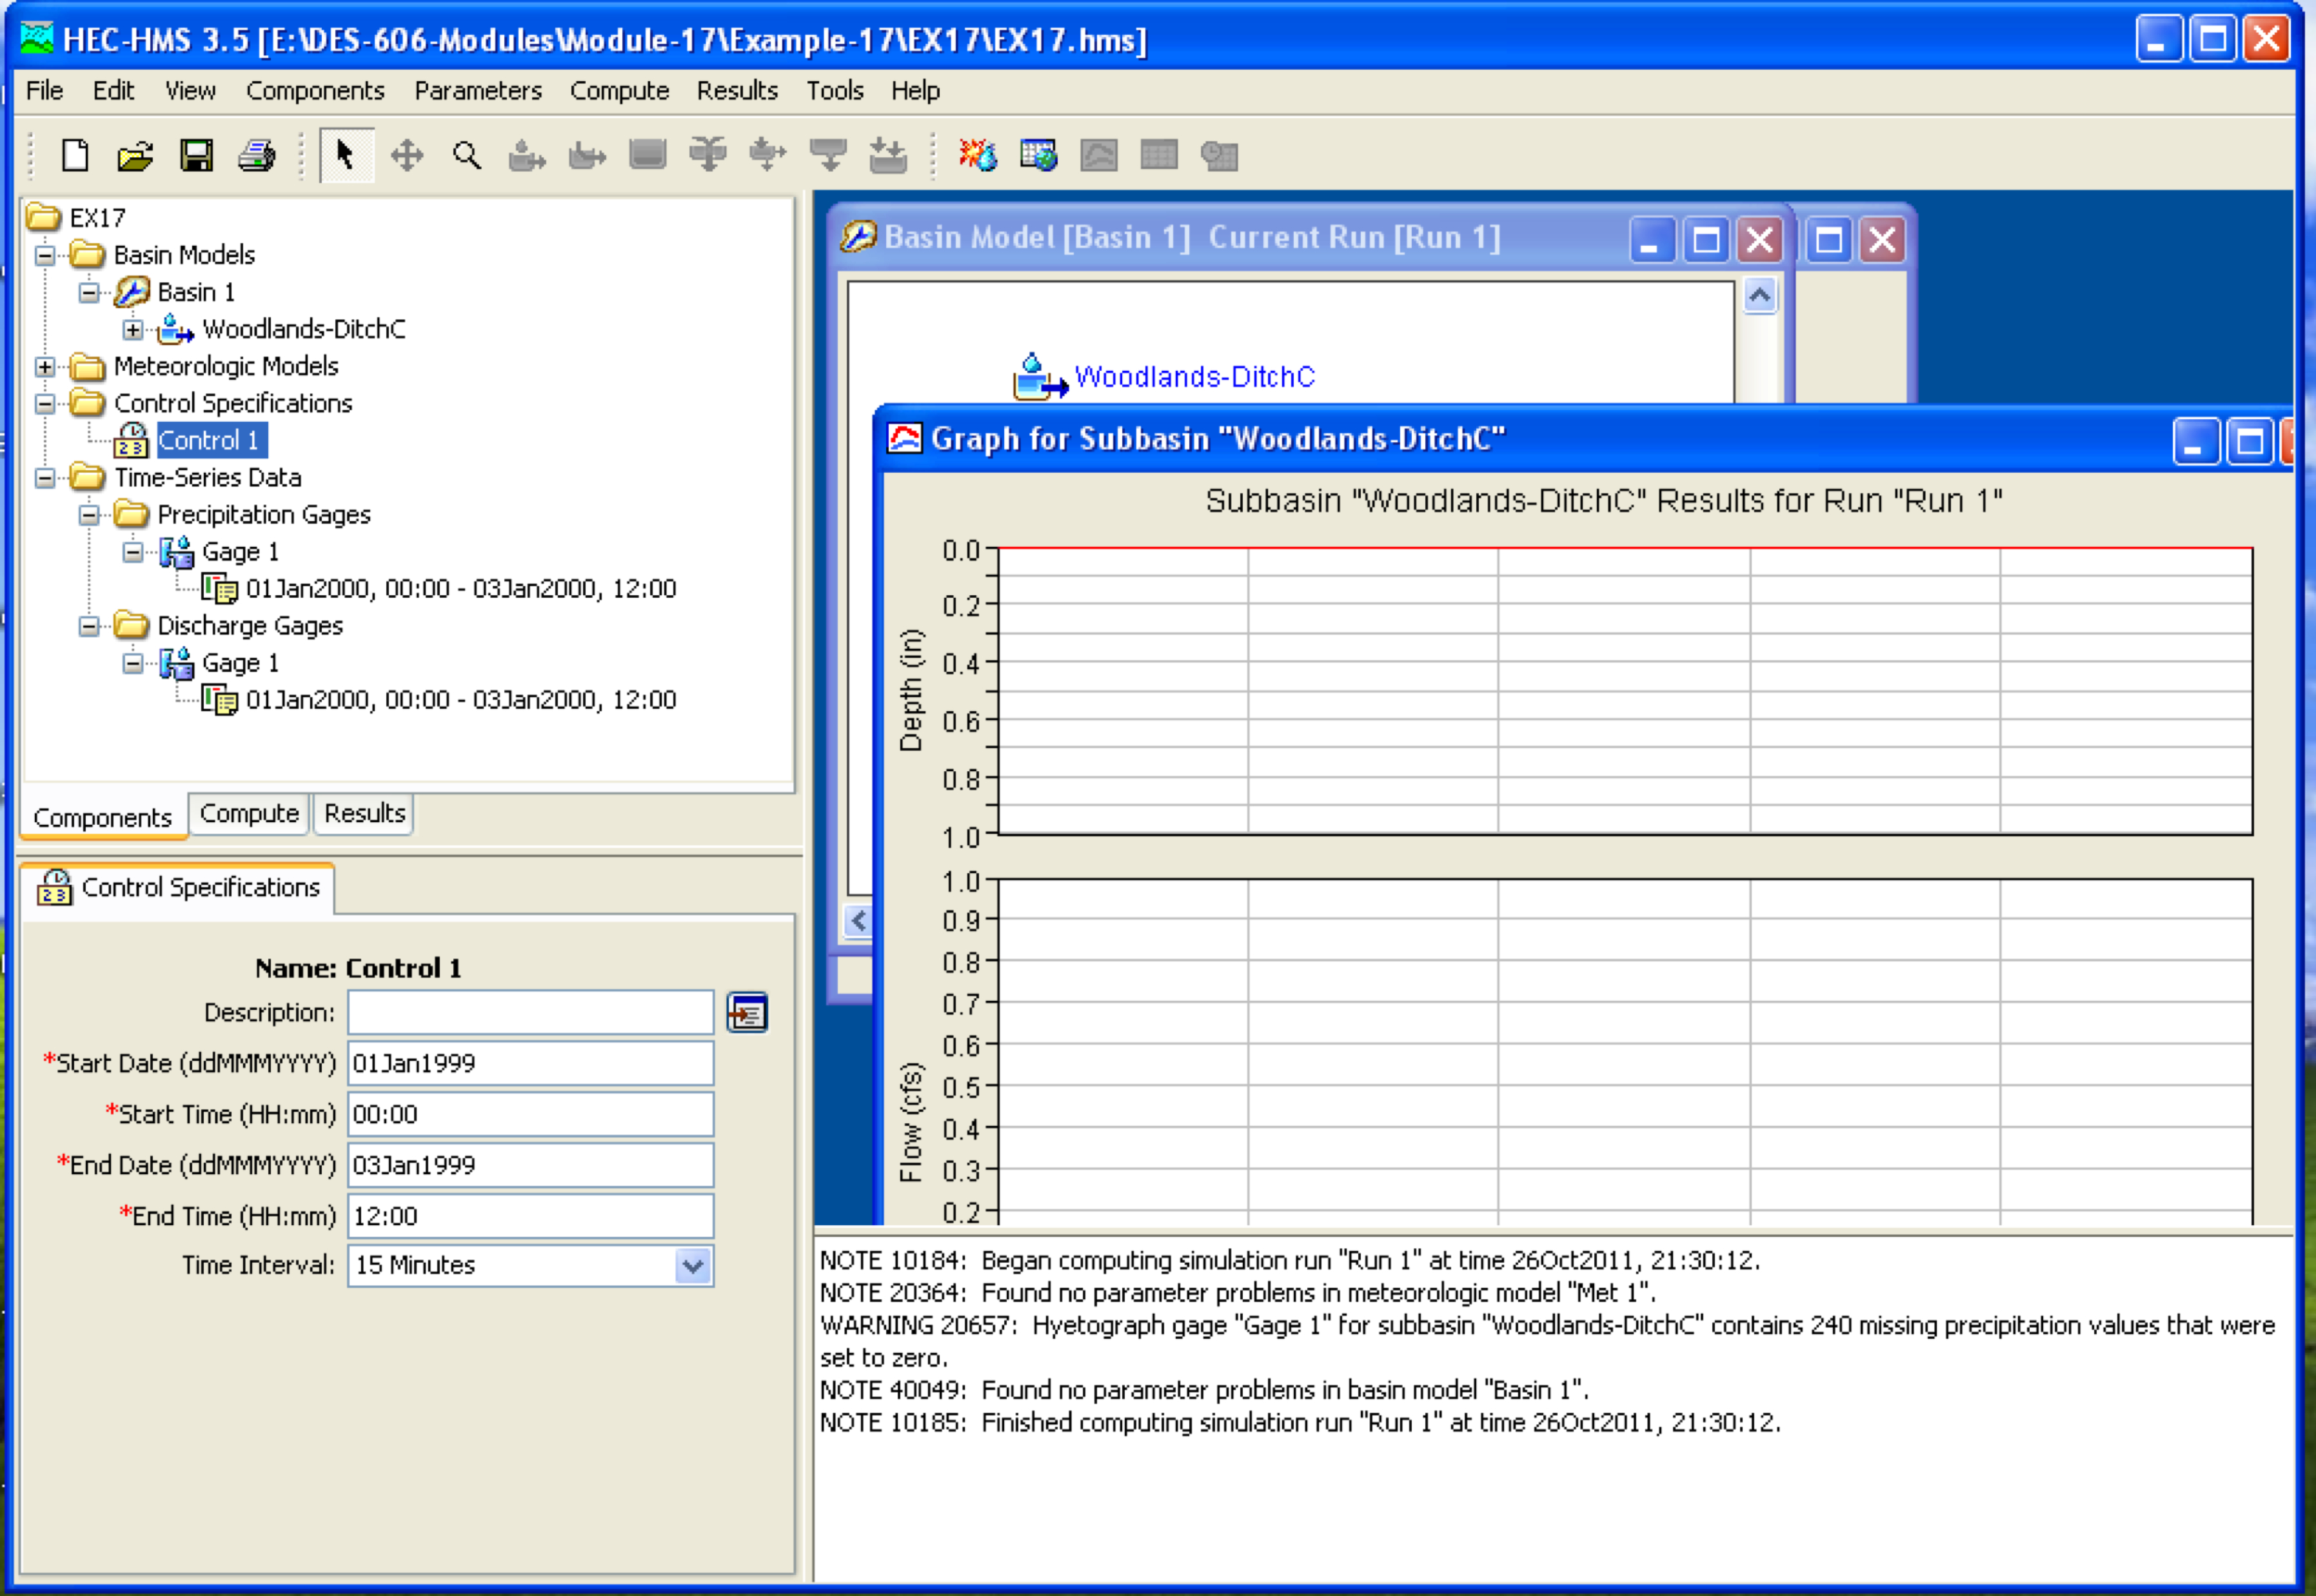
\includegraphics[width=6in]{HEC-HMS-Output3.jpg} 
   \caption{HEC-HMS Model Run for Woodlands-Ditch C sub-basin.}
   \label{fig:HEC-HMS-Output3}
\end{figure}

What is a likely explanation for the unanticipated output?

% Requires the booktabs if the memoir class is not being used
\begin{table}[h!]
   \centering
   %\topcaption{Table captions are better up top} % requires the topcapt package
\begin{tabular}{p{5in}} % Column formatting, @{} suppresses leading/trailing space
~ \\
\hline
~ \\
~ \\
\hline
~ \\
~ \\
\hline
\end{tabular}

   \label{tab:booktabs}
\end{table}
\clearpage
%%%%%%%%%%%%%%%%%%%%%%%%%%%
Figure \ref{fig:DogRun} is a schematic diagram of a creek that penetrates a 3-meter thick confined aquifer. 
During a long drought the flow in the creek \textbf{decreases} by 1.1 cubic meters per second between two gaging stations along the creek located 6 kilometers apart. 
On the west side of the creek the hydraulic head contours are parallel to the creek and the levels decrease moving \textbf{towards} from the creek at a rate of 0.0003 m/m. 
The head contours on the east side of the creek are also parallel to the creek and the levels decrease moving \textbf{away} from the creek at a rate of 0.0007 m/m.

\begin{figure}[htbp] %  figure placement: here, top, bottom, or page
   \centering
   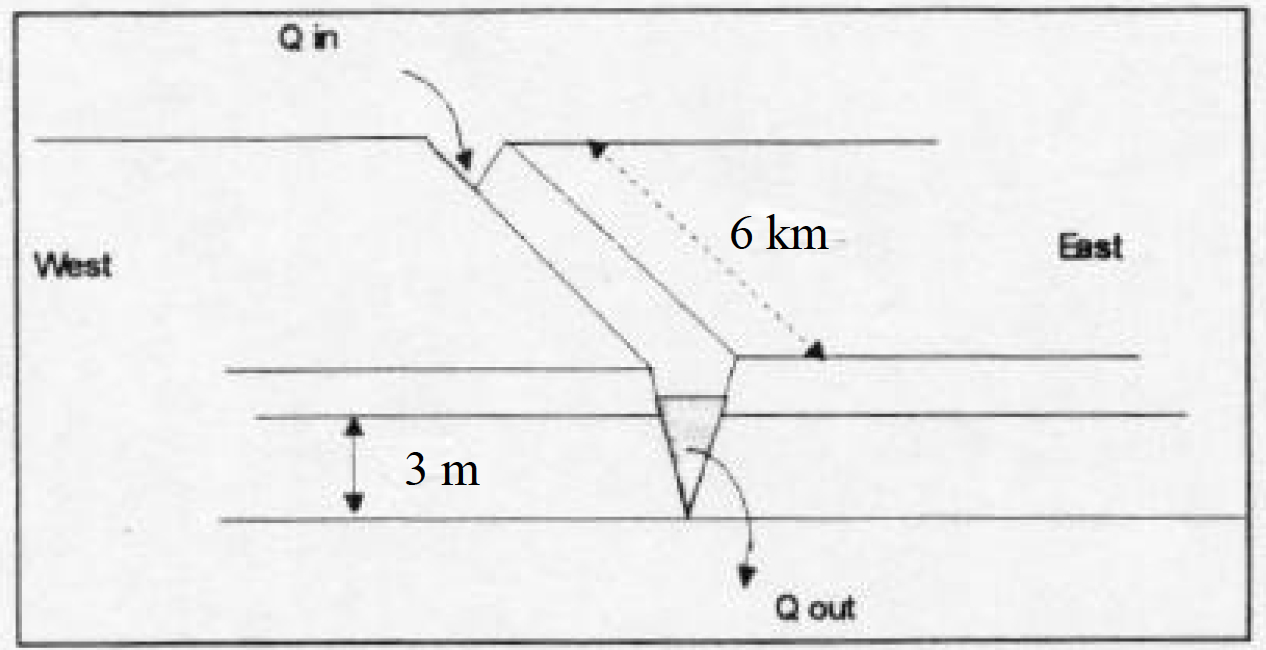
\includegraphics[width=3in]{DogRun.jpg} 
   \caption{Dog Run Creek Schematic}
   \label{fig:DogRun}
\end{figure}

\item Figure \ref{fig:DogWaterBalance} is a representative sketch of a water balance where the term $R_{in}$ represents the recharge from the stream into the aquifer.

\begin{figure}[htbp] %  figure placement: here, top, bottom, or page
   \centering
   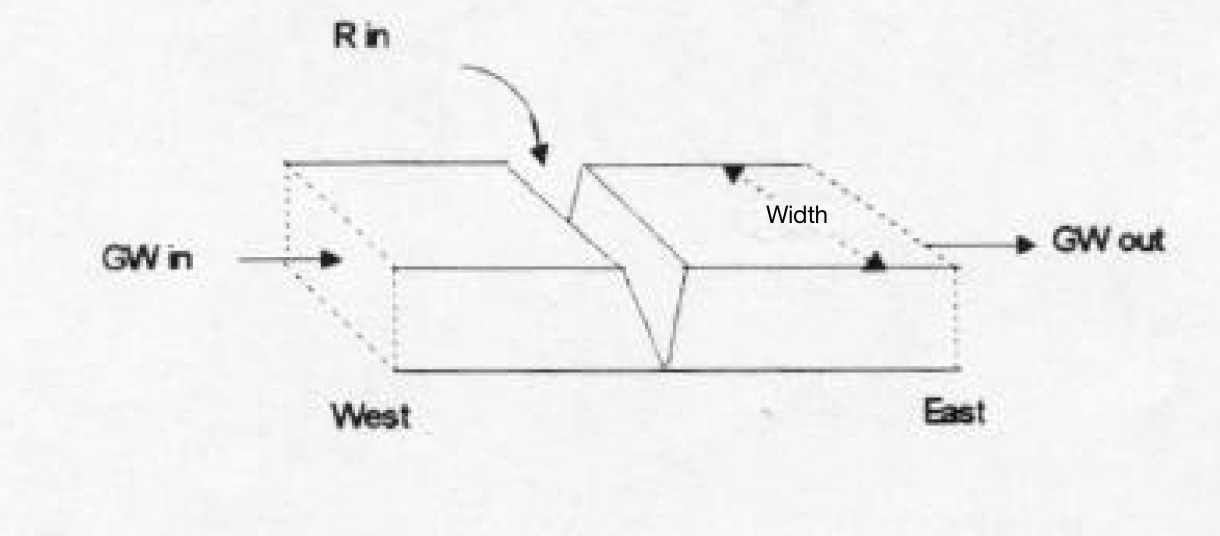
\includegraphics[width=3in]{DogWaterBalance.jpg} 
   \caption{Dog Run Water Balance}
   \label{fig:DogWaterBalance}
\end{figure}

Which expression best represents the water balance for the \textbf{aquifer} in the vicinity of the creek?
\begin{enumerate}[a)]
\item $Q_{WEST} - R_{RIVER} - Q_{EAST} = 0$ 
\item $Q_{WEST} + R_{RIVER} - Q_{EAST} = 0$ %thisone
\item $Q_{EAST} - R_{RIVER} =  Q_{EAST} $ 
\item $R_{RIVER} + Q_{WEST} = Q_{WEST} $ 
\end{enumerate}
%%%%%%%%%%%%%%%%%%%%%%%%%%%%%%%%%%%%%%%%%%%%%%
\clearpage
\item Which value using Darcy's Law and the water balance is the best estimate the hydraulic conductivity of the aquifer in Figures \ref{fig:DogRun} and \ref{fig:DogWaterBalance}?

\begin{enumerate}[a)]
\item $0.105 \frac{m}{sec}$
\item $0.153 \frac{m}{sec}$
\item $0.250 \frac{m}{sec}$
\item $0.302 \frac{m}{sec}$
\end{enumerate}


\clearpage
%%%%%%%%%%%%%%%%%%%%%%%%%%%
\item During a drought period the following declines in the water table were recorded in an unconfined aquifer.\\
% Requires the booktabs if the memoir class is not being used
\begin{table}[htbp]
\centering
  \caption{Water Table Declines}
\begin{tabular}{p{1in}p{1in}p{1in}}
Area	& Size (mi2) & Decline (ft)\\
\hline
\hline
A&	14	&2.75\\
B&	7	&3.56\\
C	&28	&5.42\\
D	&33	&7.78\\
\hline
\end{tabular}\\
   \label{tab:booktabs}
\end{table}\\
The total volume of water removed from storage in this aquifer during the time period was $5.7385 \times 10^4$ acre-feet.  
Which value below is the best estimate the specific yield of this aquifer, for the data provided?
\begin{enumerate}[a)]
\item $0.09$
\item $0.10$
\item $0.15$
\item $0.20$ %
\end{enumerate}

\clearpage

%%%%%%%%%%%%%%%%%%%%%%%%%%%
\item Three wells monitor an aquifer as shown in Figure \ref{fig:3well}.  The head in each well is listed in table \ref{tab:3well} below.   %Determine the magnitude and direction of the hydraulic gradient in this aquifer.  
\begin{table}[htbp]
\centering
  \caption{Monitoring Well Locations and Head}
\begin{tabular}{p{1in}p{1in}p{1in}p{1in}}
Area	& Size (mi2) & Decline (ft)\\
\hline
\hline
Well ID	&X	&Y	&Head\\
\#1	&10	&90	&93.2\\
\#2	&20	&5	&88\\
\#3	&90	&95	&90\\
\hline
\end{tabular}\\
\label{tab:3well}
\end{table}\\
\begin{figure}[htbp] %  figure placement: here, top, bottom, or page
   \centering
   \includegraphics[width=4in]{3well.jpg} 
   \caption{Map of well locations for Table \ref{tab:3well}}
   \label{fig:3well}
\end{figure}

Which value(s) below best represent the magnitude and direction of the hydraulic gradient in this aquifer. 
\begin{enumerate}[a)]
\item $\frac{\Delta h}{\Delta L}~\approx 0.084; NW to SE$
\item $\frac{\Delta h}{\Delta L}~\approx 0.384; NW to SE$
\item $\frac{\Delta h}{\Delta L}~\approx 0.084; NE to SW$
\item $\frac{\Delta h}{\Delta L}~\approx 0.384; NW to SE$ %
\end{enumerate}
\clearpage
%%%%%%%%%%%%%%%%%%%%%%%
\item An unconfined aquifer is 300 feet deep, and has a hydraulic conductivity of 0.5 feet per day.
A one-foot diameter well is drilled into the aquifer an pumped at a rate of 50 gallons per minute.
The well's radius of influence is 1000 feet. After pumping has continued long enough for equilibrium to be established, the depth of water in the well is
%standard answer set
\begin{enumerate} [a)]
\item $190$ feet
\item $220$ feet
\item $240$ feet
\item $270$ feet
\end{enumerate}
\clearpage
%%%%%%%%%%%%%%%%%%%%%%
\item Figure \ref{fig:debrisDam} depicts a concrete dam that impounds water as shown.  
The standing water depth is 1.5 meters.
The soil layer under the reservoir is underlain by a highly porous sand layer.
\begin{figure}[h!] %  figure placement: here, top, bottom, or page
\centering
   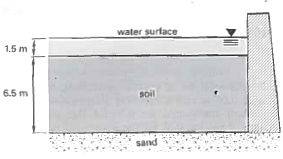
\includegraphics[width=3in]{dam.jpg}
   \caption{Debris trap (dam) with 6.5 meters of sediment above a sand layer}
   \label{fig:debrisDam} 
\end{figure}
The sand layer at the bottom of the soil profile has horizontal drainage and zero pore pressure.
The water level of the reservoir is constant.
The total surface area of the reservoir pool is 1000 m$^2$, and the hydraulic conductivity of the soil layer is 4.7$\times$10$^{-6}$ mm/sec.
The loss from seepage through the soil layer per year is
%standard answer set
\begin{enumerate} [(A)]
\item $1.1$ cubic meters
\item $2.8$ cubic meters
\item $34$ cubic meters
\item $180$ cubic meters
\end{enumerate}

%%%%%%%%%%%%%%%%%%%%%%%%%%%
\end{enumerate}
\end{document}


